\documentclass[letter]{ieicej}
\usepackage[dvipdfmx]{graphicx,xcolor}
\usepackage[fleqn]{amsmath}
\usepackage{newtxtext}
\usepackage[varg]{newtxmath}
\usepackage{url}
\makeatletter\def\hyper@nopatch@bib{}\makeatother
\usepackage[dvipdfmx,hidelinks]{hyperref}
\typeofletter{研究速報}
\field{}
\jtitle{LLMエージェントの履歴要約と終了制御による\\実行費用の評価}
\etitle{Evaluating Execution Cost of History Summarization and Termination Control for LLM Agents}
\authorlist{%
\authorentry[tp26013-0852@sti.chubu.ac.jp]{桐生 篤希}{Atsuki KIRYU}{s}{chubu}\MembershipNumber{}
\authorentry{菊澤 百々菜}{Momona KIKUZAWA}{s}{chubu}\MembershipNumber{}
\authorentry{木村 秀明}{Hideaki KIMURA}{f}{chubu}\MembershipNumber{}
}
\affiliate[chubu]{中部大学大学院工学研究科情報工学専攻，愛知県}{Department of Computer Science, Graduate School of Engineering, Chubu University, 1200 Matsumoto-cho, Aichi, 487-0027 Japan}
\alignorder=1\relax
\jalcdoi{???????????}
\clubpenalty=10000
\widowpenalty=10000
\raggedbottom
\begin{document}
\maketitle
\begin{abstract}
LLMエージェントの履歴要約方式とAPI実行記録に基づく終了制御を独立に評価する．要約生成を含む全モデル呼出しを計測し，今回の既知課題で成功を保ちながら総トークン数が減少したことを確認した．呼出し配置と完了後の生成に着目した比較結果を示す．
\end{abstract}
\begin{keyword}
LLMエージェント，ハーネス，履歴要約，終了制御，トークン使用量
\end{keyword}
\begin{eabstract}
We independently evaluated history summarization methods and termination control based on API execution records for LLM agents. Counting all model calls, including dedicated summarization, showed reductions in total tokens while preserving success on known tasks under the evaluated conditions.
\end{eabstract}
\begin{ekeyword}
LLM agents, harness, history summarization, termination control, token usage
\end{ekeyword}

% Single-column tables; scientific values unchanged from v08.
\newcommand{\SummaryResultsTable}{%
\begin{table}[!ht]
\caption{実験Aの課題別総トークン数}
\label{tab:summary}
\centering\fontsize{7}{9}\selectfont
\begin{tabular*}{65mm}{@{\extracolsep{\fill}}lrrr@{}}\hline
課題 & \shortstack{専用1回\\方式} & \shortstack{専用反復\\方式} & \shortstack{行動併記\\方式}\\\hline
写真操作 & 139,871 & 139,871 & 129,374\\
精算 & 211,110 & 211,110 & 211,110\\
返金 & 102,087 & 102,087 & 102,087\\
CSV処理 & 440,461 & 332,588 & 394,351\\\hline
合計 & 893,529 & 785,656 & 836,922\\\hline
\end{tabular*}
\end{table}}

\newcommand{\TerminationResultsTable}{%
\begin{table}[!ht]
\caption{実験Bの総トークン数と呼出し回数}
\label{tab:termination}
\centering\fontsize{7}{9}\selectfont
\begin{tabular*}{65mm}{@{\extracolsep{\fill}}llrrr@{}}\hline
API条件 & 終了方法 & 総トークン数 & \shortstack{モデル\\呼出し数} & \shortstack{API\\要求数}\\\hline
文書必須 & 通常継続 & 130,439 & 15 & 104\\
文書必須 & 終了制御 & 91,116 & 13 & 100\\[2pt]
名前参照 & 通常継続 & 151,664 & 14 & 103\\
名前参照 & 終了制御 & 112,233 & 12 & 99\\\hline
\end{tabular*}
\end{table}}


\section{はじめに}

日常業務のデータ整理や事務処理を支援する大規模言語モデル（LLM）の研究が進んでいる．写真整理や精算では，文章生成に加え，外部アプリケーションで対象の検索，状態の変更，結果の確認を連続して行う必要がある．推論と行動を繰り返すReAct\cite{yao2023react}や，コードを行動として実行するCodeAct\cite{wang2024codeact}は，こうした処理を支える．

しかし，実行が長期化すると，過去の操作や観測結果を次の生成へ繰り返し入力する費用が増大する．また，作業が完了した後もエージェントが確認や生成を続ければ，成果を増やさずに計算資源を消費し得る．単純に履歴を短縮するだけでは課題の遂行に必要な情報を失うおそれがあり，一方で早期に終了させれば課題が未完了に終わるおそれがある．そのため，課題の最終的な成功と実行全体の費用を同時に検証する必要がある．

そこで本稿では，モデルの再学習を伴わずに実行を管理するハーネスを用い，履歴要約の呼出し配置と終了制御を評価する．履歴要約では，要約を生成する時点，行動生成と要約の呼出しを分けるかどうか，要約機会の上限を比較軸とする．また，終了制御では，実行中に取得できるAPIの要求と応答を記録し，このAPI実行記録に基づく制御を通常継続と比較する．両者を独立した実験として実施し，要約生成を含む全モデル呼出しの総トークン数と，課題の最終的な成功を調べる．

\par\noindent\begin{minipage}{\columnwidth}
\section{関連研究}

入力圧縮の分野では，長文中の情報の位置が性能に影響すること\cite{liu2024lost}を踏まえ，LLMLingua\cite{jiang2023llmlingua}が予算制御とトークン選別を，LLMLingua-2\cite{pan2024llmlingua2}が蒸留データによるトークン分類を，LongLLMLingua\cite{jiang2024longllmlingua}が長文の重要情報を残す圧縮をそれぞれ扱っている．

\end{minipage}\par\penalty0

長期実行の観点では，ACON\cite{kang2026acon}が観測・履歴の圧縮方針を，TokenPilot\cite{xu2026tokenpilot}が入力圧縮とキャッシュ継続性を検討している．さらに，Generative Agents\cite{park2023generative}は経験の記憶・抽象化・検索を，Reflexion\cite{shinn2023reflexion}は言語的フィードバックを後続試行に利用する手法を扱っている．本稿では，要約専用の呼出しを用いる方式と，行動と同じ応答内に含める方式を比較し，要約生成も含めた課題全体のトークン使用量を評価する．

一方，終了制御に関しては，Runaway\cite{lu2025runaway}が終了指示と外部の完了検証を検討している．本稿では，既知の要求形式についてAPI実行記録から完了条件を検査する．通常継続との比較を通じて，課題の最終的な成功，API要求数，総トークン数を評価する．

\section{提案手法}

ハーネスとは，モデルの外側で入力と実行の継続を管理するプログラムを指す．本稿では，既存の要約を用いて入力履歴を更新する処理と，API実行記録に基づいて次の生成の要否を判断する処理をそれぞれ構成する．図\ref{fig:architecture}の実験Aに要約と行動生成の呼出し配置を，実験Bに完了判定に基づく終了制御を示す．両者は個別に評価し，組合せによる削減効果は本稿の対象外とする．

専用1回方式と専用反復方式では，行動と要約の呼出しを分ける構成を共通とし，要約機会の上限を比較する．専用反復方式と行動併記方式では，機会の上限を揃え，要約候補を専用呼出しで生成するか，行動と同じ応答に含めるかを比較する．候補の採否と入力の更新は，いずれもモデルの外側のハーネスが担う．

まず，課題と履歴からモデルが行動を生成し，ハーネスがプログラムを実行して行動と結果を記録する．本稿では，行動生成から実行結果の記録までを1ターンと定義する．

% Figure 1 begins the next page; subsection 3.1 follows beneath it.
\twocolumn[{%
\begin{minipage}{\textwidth}
\centering
\expandafter\def\csname @captype\endcsname{figure}
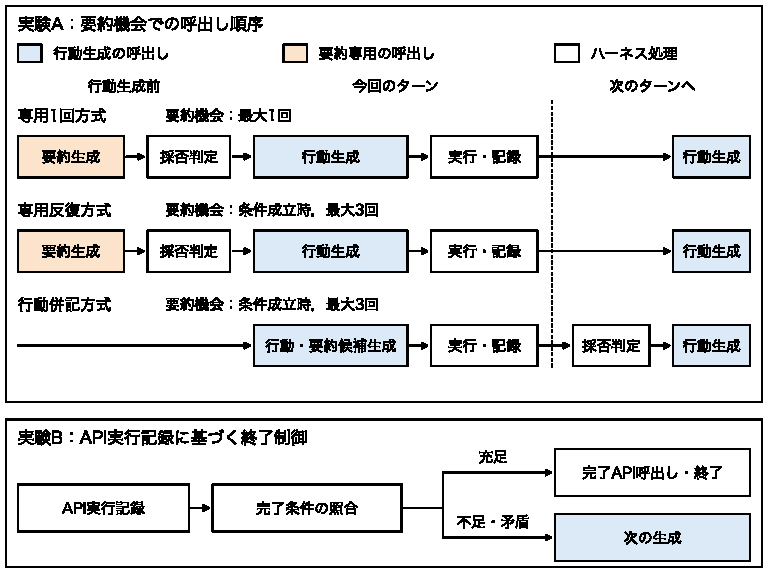
\includegraphics[width=130mm]{figures/control_points.pdf}
\capwidth=130mm\ecapwidth=130mm
\abovecaptionskip=1pt\belowcaptionskip=1pt
\caption{履歴要約方式と終了制御}
\label{fig:architecture}
\end{minipage}%
}]

\subsection{入力履歴を短くする制御}

履歴の蓄積による入力の長大化を抑えるため，保存した全履歴は維持しつつ，モデルへ渡す古い履歴を要約に置き換える．生成された要約のうち，検査を経て採用される前のものを要約候補と呼ぶ．本稿では，要約の生成のみを目的とするモデル呼出しを専用呼出しと定義し，以下の3方式に比較用の名称を付ける．

専用1回方式は，要約専用のモデル呼出しを最大1回追加する方式である．入力長が閾値に達し，かつ要約可能な古い履歴が存在する最初の機会に候補を生成する．候補を検査して採用した場合は，要約と未要約の履歴を次の行動生成へ渡す．要約機会は最大1回とし，その機会が終了した後は新たな要約を試みない．

専用反復方式は，要約専用の呼出しを必要に応じて繰り返す方式である．最初の要約機会では専用1回方式と同じ処理を行う．それ以降は，入力長と新たに完了したターン数の条件を満たすたびに，その時点で未要約の古い履歴を要約対象とする．採用済みの要約が存在する場合は，それも新たな要約対象に含める．要約機会は最大3回とし，各機会で候補の採否を決定してから次の行動生成へ進む．

行動併記方式は，行動を生成するモデルの同じ応答内に，行動と要約候補を出力させる方式である．要約専用の呼出しは追加せず，最大3回の要約機会を設ける．この方式では，応答内の全プログラムを実行して結果を記録した後，次の行動生成へ進む前に候補の採否を決定する．ただし，候補には同じ応答で生成した行動の実行結果を含めない．その行動と結果は原文のまま次の入力に残す．

どの方式でも，要約には完了した作業，次の操作に使う情報，残作業，不確かな点の四つの欄を設ける．要約候補が得られた際，ハーネスはまず形式と文字数を検査する．さらに，元の指示と課題，要約，未要約の履歴を含めた次回入力全体のトークン数を算出し，候補を採用しない場合より厳密に少なくなることを確認して採用する．要約候補を生成する時点では，直近2ターンを原文のまま保持する．ここで検査するのは構造と入力長であり，要約内容の正確性を保証するものではない．

具体的には，完了した作業の欄には実行済みの内容を，次の操作に使う情報の欄には識別子やAPIの呼出し方，保持された変数などを残すよう指示する．一方，残作業と不確かな点の欄では，未実施の操作と未確認の事項を区別させる．また，APIの正常応答だけを根拠に課題の完了を推定しないよう求める．

元の指示と課題は要求の基準として保持し，直近の行動とAPI応答も原文のまま渡す．これにより，古い履歴の提示方法を圧縮しつつ，要求内容と直近の実行結果を参照できる構成とする．

採用条件を満たさなかった場合は，それまでの要約と未要約の履歴を維持する．まだ一度も要約を採用していない段階では，要約前の履歴をそのまま使い続ける．要約機会とは候補の生成を試みる機会を指し，採用回数とは区別する．不採用の場合も1回の機会として数え，その場での再生成は行わない．専用1回方式は機会の上限を定める名称であり，生成や採用が0回となる場合もある．入力長とターン数の閾値は4.1に示す．保存した全履歴は，入力を短縮した後も別に保持する．

専用呼出しを用いる方式では，候補生成に1回のモデル呼出しを要する．一方，行動併記方式では行動生成の呼出しを共有する．採用回数は，候補を採用して入力を実際に更新した回数を指す．本稿では，要約機会数，採用回数，モデル呼出し数を明確に区別して扱う．また，要約の採用後も，新たな行動と結果は未要約の履歴として追加され，次の要約機会まで入力に残る．

\subsection{作業完了後の生成を省く制御}

終了制御とは，API実行記録から課題の完了状況を検査し，根拠が揃った時点で次の生成を省く処理である．本稿では，この検査段階を完了判定と呼ぶ．写真を作成時期に応じた指定先へ移す課題を対象とし，既知の一つの要求形式に対応する検査規則を手書きで用意する．まず，モデル応答内の全プログラムを実行し，APIの要求と応答を記録する．次に，移動前の写真一覧，各写真の作成日時，APIから取得した現在年を確認する．これらの情報に基づき，全ての対象写真が指定先へ移動し，元の名前が保たれているかを照合する．完了の根拠が初めて揃った時点で完了APIを1回呼び出し，次の生成を省く．

この完了判定はモデル自身の完了宣言に依存せず，API実行記録に対象全件の処理を確認できる情報が含まれているかを調べる．比較対象となる通常継続では，この判定による終了を行わず，通常の実行手順を続ける．

移動前に対象集合を確定させるのは，一部の写真の移動だけで完了と判断することを避けるためである．作成日時とAPIから取得した現在年は，写真ごとに指定された移動先を照合する際に使う．また，移動後の場所に加えて元の名前の保持を調べることで，指定先へ移すという要求と，名前を変えないという要求を別々に確認する．これらの根拠はモデルの推測や計算機の時刻では補わず，API実行記録から取得する．

対応する要求形式から外れる場合や，判定に必要な記録が不足・矛盾している場合には，通常どおり次の生成へ進む．判定には，その時点で得られたAPI実行記録のみを使用し，公式評価器の正解は利用しない．履歴要約との組合せ効果は評価しない．

\subsection{総トークン数と課題の成功}

1回あたりの入力を短縮しても，要約生成やその後の行動生成に使用するトークンが増えれば，課題全体の使用量は増加し得る．そのため，要約後の入力長だけを比較せず，課題開始から終了までを全方式に共通する集計範囲とする．

\par\noindent\begin{minipage}{\columnwidth}
\setlength{\abovedisplayskip}{4pt}\setlength{\belowdisplayskip}{4pt}
条件$p$で実行したモデル呼出しの集合を$\mathcal C_p$とする．各呼出し$c$の入力トークン数を$I_c$，出力トークン数を$O_c$とし，実行全体の総トークン数$T_p$を\mbox{式\eqref{eq:cost}で求める．}

\begin{equation}
 T_p=\sum_{c\in\mathcal C_p}(I_c+O_c)
 \label{eq:cost}
\end{equation}

要約処理自体にも生成費用がかかるため，行動生成と要約生成の両方を合算して集計する．不採用となった要約候補の生成や，失敗時の呼出しについても，取得できた使用量は全て計上する．使用量が不明な場合は0とせず，既知分の小計と不明件数を記録する．

\end{minipage}\par\penalty0

課題の成功は，実行終了後の最終状態に対してAppWorld\cite{trivedi2024appworld}の公式評価器を用いて判定する．評価器の正解や詳細情報は，実行中のモデルへ返さない．方式間では成功数に加え，各課題の成功が維持されているかを確認する．

同じ課題を処理した方式同士で成功と総トークン数を対応させる．課題をまたぐ合計では減少と増加が相殺されるため，実験Aでは課題別の値も示す．

本指標はキャッシュされた入力も含む論理トークン数であり，金銭的な課金や実際の実行時間を直接表すものではない\cite{xu2026tokenpilot}．要約生成を含む費用評価はACON\cite{kang2026acon}にも用いられている．実験AとBは独立に集計する．履歴要約は次回入力の長さを，終了制御は次の生成の必要性を管理する．判断材料と変更対象が異なるため，それぞれの制御と対照を独立に比較する．

\section{実験A：要約の呼出し配置}

\subsection{条件}

写真操作，精算，返金，CSV処理の既知4課題に対し，専用1回方式，専用反復方式，行動併記方式の各方式を各課題で1回ずつ実行した．4課題に3方式を適用し，計12実行とした．モデルは全条件でMiniMax-M3を用い，GGUF形式のIQ4\_XS量子化モデルをllama.cpp b11669で実行した．文脈長は65,536トークンである．乱数の初期値を表すseedは，モデル生成の基点を57，環境を42とした．生成側は呼出しの役割と順序に従いseedを増分した．

要約機会を設ける入力長の閾値は16,384トークンとし，要約時には直近2ターンを原文のまま保持する．専用反復方式と行動併記方式では，前回の要約機会が終了してから新たに3ターン以上が完了することを要求する．採用と不採用のどちらでも，その機会の終了時点を次回の起点とする．初回の起点は課題開始である．要約は合計8,192文字以下とし，次の行動生成へ渡す入力全体が短くなる場合に採用する．要約専用の呼出しでは出力上限を4,096トークンとし，その使用量も式\eqref{eq:cost}へ含める．

各実行の上限はモデル呼出し80回，総トークン数450,000，作業時間1,800秒とし，環境APIは写真160，他3課題80要求とした．生成の温度は行動生成で1.0，要約専用の生成で0.7とした．並列実行数は1，KVキャッシュはq8\_0，計算機はApple M3 Ultra，メモリは256 GiBである．実装と記録を公開する\footnote{\url{https://github.com/sophiria1225/AI-}}．

\subsection{全4課題の結果}

表\ref{tab:summary}に4課題の結果を示す．全12実行で課題の成功を確認し，使用量の欠測はなかった．

\SummaryResultsTable

要約生成を含む4課題の合計では，専用反復方式が785,656トークンで3方式中最少となった．専用1回方式の893,529トークンと比較して107,873トークン少なく，削減率は12.07\%であった．ただし，この差はCSV処理のみで生じており，残る3課題では両方式の値が一致した．

写真操作では，専用1回方式と専用反復方式が139,871トークンであったのに対し，行動併記方式は129,374トークンとなった．行動併記方式は他の2方式より10,497トークン少なかった．要約の採用回数はいずれも1回であったが，同じ採用回数でも課題全体の総トークン数には差が生じた．

一方，精算の総トークン数は全方式で211,110トークンであった．要約の採用回数はいずれも0回であり，方式による総量の差は見られなかった．

返金では，全方式で102,087トークンを使用し，要約の採用回数は0回であった．精算と同様に，成功と総トークン数は全方式で一致した．

CSV処理では，専用1回方式が440,461，専用反復方式が332,588，行動併記方式が394,351トークンであった．専用反復方式は専用1回方式より107,873トークン少なく，4課題合計での削減はこの課題で生じた．要約の採用回数は専用1回方式が1回，専用反復方式と行動併記方式が各2回であった．専用反復方式と行動併記方式は採用回数が等しかったものの，総トークン数は一致しなかった．

行動併記方式は，4課題合計で専用1回方式より6.34\%少なかったものの，専用反復方式より51,266トークン多く，増加率は6.53\%であった．専用反復方式との比較では，写真操作で10,497トークン減少した一方，CSV処理で61,763トークン増加した．要約専用の呼出しを省く構成でも，今回の条件では課題全体の総トークン数が最少になるとは限らなかった．表\ref{tab:summary}に課題別の値と合計を併記することで，異なる課題で生じた減少と増加を分けて確認できる．

\section{実験B：API実行記録に基づく終了制御}

\subsection{条件}

同じ写真課題について，API文書の取得を必須とする文書必須条件と，公開API名からのアクセスを許す名前参照条件を設けた．各条件で，通常継続と，API実行記録に基づく終了制御を比較した．終了制御は，事前に実行・保存した通常継続と同じ初期状態，モデル，seed，モデルへの指示とツール説明，予算を用いて各1回実行した．

seedの基点は42であり，実験Aとは別の履歴・設定である．同じMiniMax-M3 IQ4\_XSとllama.cpp b11669を用い，各実行の予算はモデル呼出し80回，450,000トークン，1,800秒，API160要求とした．

完了判定と完了通知は3.2に従う．判定，記録保存，完了通知を含む実行時間を記録し，完了通知をAPI要求数に含めた．

行動の生成はLLMが担い，記録の検査はハーネスの規則で行う．この検査のために別のモデル呼出しは設けない．完了の根拠が揃えば次の行動生成を省き，根拠が足りなければ同じ実行を継続する．

終了以前の生成過程の違いが比較に含まれていないか確認するため，終了制御側で実行したモデル呼出しの要求と応答が，通常継続側の先頭から同じ範囲と完全に一致することを事前の照合基準とした．API操作の記録と最終状態も比較した．

\subsection{成功を保った総トークン数の削減}

表\ref{tab:termination}に結果を示す．両API条件で，終了制御を用いた実行は課題の成功を保ち，通常継続より総トークン数が少なかった．文書必須条件では130,439から91,116へ30.15\%，名前参照条件では151,664から112,233へ26.00\%減少した．全4実行で公式評価器による成功を確認し，使用量の欠測はなかった．各条件で，モデル呼出しは2回，API要求は4回減少した．完了通知を含めて処理を終えた実行では，移動後の確認API4回と，それに伴う生成が省かれた．

\TerminationResultsTable

\par\noindent\begin{minipage}{\columnwidth}
実行したAPI操作などの前半の記録と，実行終了時の13個のデータベースのハッシュ値は通常継続と一致し，最終状態を保った総トークン数の減少を確認した．ただし，要求・モデル応答全文の完全一致基準は満たさなかった．このため，観測された差の全てを終了制御のみの効果とは断定せず，既知の要求形式に対する各1回の比較結果として扱う．平均的な因果効果や汎用的な終了保証を示す評価ではない．
\end{minipage}\par\penalty0

\section{むすび}

既知の4課題全てで成功を保ち，専用反復方式の総トークン数は専用1回方式を12.07\%下回った．この差はCSV処理のみで生じ，他3課題の値は一致した．また，行動併記方式の合計は専用反復方式より6.53\%多かった．独立に評価した写真課題の二つのAPI条件では，終了制御を用いた実行で成功を保ち，通常継続に比べて26.00--30.15\%の削減を確認した．これらの結果は，要約生成を含む全モデル呼出しの計測と，API実行記録から得られる完了の根拠に基づく実行管理の意義を示す．

本稿は，既知課題と単一モデル・量子化設定における少数のseed・試行による開発実験を事後に整理した評価である．未見課題の品質維持や統計的非劣性は評価していない．

% Twelve formal conference/journal papers. Source verification: reference_update.json.
\begin{thebibliography}{99}
\bibitem{yao2023react}
S. Yao, J. Zhao, D. Yu, N. Du, I. Shafran, K. Narasimhan, and Y. Cao,
``ReAct: Synergizing reasoning and acting in language models,''
Proc. ICLR, May 2023.

\bibitem{wang2024codeact}
X. Wang, Y. Chen, L. Yuan, Y. Zhang, Y. Li, H. Peng, and H. Ji,
``Executable code actions elicit better LLM agents,''
Proc. ICML, PMLR, vol.235, pp.50208--50232, July 2024.

\bibitem{liu2024lost}
N. F. Liu, K. Lin, J. Hewitt, A. Paranjape, M. Bevilacqua, F. Petroni, and P. Liang,
``Lost in the middle: How language models use long contexts,''
Trans. ACL, vol.12, pp.157--173, 2024.
doi: 10.1162/tacl\_a\_00638.

\bibitem{jiang2023llmlingua}
H. Jiang, Q. Wu, C.-Y. Lin, Y. Yang, and L. Qiu,
``LLMLingua: Compressing prompts for accelerated inference of large language models,''
Proc. EMNLP, pp.13358--13376, Dec. 2023.
doi: 10.18653/v1/2023.emnlp-main.825.

\bibitem{pan2024llmlingua2}
Z. Pan, Q. Wu, H. Jiang, M. Xia, X. Luo, J. Zhang, Q. Lin, V. R\"uhle,
Y. Yang, C.-Y. Lin, H. V. Zhao, L. Qiu, and D. Zhang,
``LLMLingua-2: Data distillation for efficient and faithful task-agnostic prompt compression,''
Findings of ACL: ACL 2024, pp.963--981, Aug. 2024.
doi: 10.18653/v1/2024.findings-acl.57.

\bibitem{jiang2024longllmlingua}
H. Jiang, Q. Wu, X. Luo, D. Li, C.-Y. Lin, Y. Yang, and L. Qiu,
``LongLLMLingua: Accelerating and enhancing LLMs in long context scenarios via prompt compression,''
Proc. ACL, vol.1, pp.1658--1677, Aug. 2024.
doi: 10.18653/v1/2024.acl-long.91.

\bibitem{kang2026acon}
M. Kang, W.-N. Chen, D. Han, H. A. Inan, L. Wutschitz, Y. Chen,
R. Sim, and S. Rajmohan,
``ACON: Optimizing context compression for long-horizon LLM agents,''
Proc. ICML, PMLR, vol.306, pp.55321--55375, July 2026.

\bibitem{xu2026tokenpilot}
B. Xu, Z. Xue, D. Chen, C. Fu, C. Wu, C. Huang, C. Jiang, J. Fang,
X. Deng, Y. Chen, Y. Yao, X. Wang, J. Shang, H. Chen, and N. Zhang,
``TokenPilot: Cache-efficient context management for LLM agents,''
Findings of ACL: EMNLP 2026, pp.19034--19049, Oct. 2026.

\bibitem{park2023generative}
J. S. Park, J. O'Brien, C. J. Cai, M. R. Morris, P. Liang, and M. S. Bernstein,
``Generative agents: Interactive simulacra of human behavior,''
Proc. ACM UIST, article 2, pp.1--22, Oct. 2023.
doi: 10.1145/3586183.3606763.

\bibitem{shinn2023reflexion}
N. Shinn, F. Cassano, A. Gopinath, K. Narasimhan, and S. Yao,
``Reflexion: Language agents with verbal reinforcement learning,''
Advances in Neural Information Processing Systems, vol.36, pp.8634--8652, 2023.
doi: 10.52202/075280-0377.

\bibitem{lu2025runaway}
Q. Lu, L. Ding, S. Cao, X. Liu, K. Zhang, J. Zhang, and D. Tao,
``Runaway is ashamed, but helpful: On the early-exit behavior of large language model-based agents in embodied environments,''
Findings of ACL: EMNLP 2025, pp.24014--24027, Nov. 2025.
doi: 10.18653/v1/2025.findings-emnlp.1304.

\bibitem{trivedi2024appworld}
H. Trivedi, T. Khot, M. Hartmann, R. Manku, V. Dong, E. Li, S. Gupta,
A. Sabharwal, and N. Balasubramanian,
``AppWorld: A controllable world of apps and people for benchmarking interactive coding agents,''
Proc. ACL, vol.1, pp.16022--16076, Aug. 2024.
doi: 10.18653/v1/2024.acl-long.850.

\end{thebibliography}

\end{document}
